\documentclass[fleqn]{jbook}
\usepackage{physpub}

\begin{document}

\begin{question}{専攻 問題1}{}

中心対称場の中の粒子の運動に対するシュレディンガー方程式は次のように与えられる。
\[ \frac{\hbar^2}{2m}\Delta \Psi+[E-U(r)]\Psi =0 \]
ここで$m$および$E$はそれぞれ粒子の質量とエネルギー、また$U(r)$は場のポテンシャルエネルギーである。ラプラス演算子$\Delta$は
\[ \Delta\equiv\frac{\partial^2}{\partial x^2}+\frac{\partial^2}{\partial y^2}+\frac{\partial^2}{\partial z^2} \]
で、$r=\sqrt{x^2+y^2+z^2}$である。

中心対称場の中の運動では角運動量が保存されるので、波動関数$\Psi$の動径関数$R_l(r)$は次の方程式を満たす。
\[\frac{1}{r^2}\frac{d}{dr}\left(r^2\frac{dR_l}{dr}\right)-\frac{l(l+1)}{r^2}R_l+\frac{2m}{\hbar^2}[E-U(r)]R_l=0 \]
ここで$l$は粒子の角運動量である。以下では角運動量$l=0$の動径関数$R_0(r)$について考えよう。

\begin{subquestions}
\SubQuestion
井戸型ポテンシャル
\[ 
U(r)=\left\{ 
\begin{array}{rcc}
-U_0 & , & r \leq r_0 \\
0    & , & r > r_0  
\end{array}
\right.
\]
において、以下の問いに答えよ。ただし、$U_0$は正の定数で$-U_0\leq E \leq 0$とする。
\begin{subsubquestions}
\SubSubQuestion
$r\leq r_0$での$R_0(r)$の形を求めよ。
\SubSubQuestion
$r>r_0$での$R_0(r)$の形を求めよ。
\SubSubQuestion
上記の(i)と(ii)で求めた動径関数$R_0(r)$を$r=r_0$でなめらかにつなぎ、粒子のエネルギー$E$と$r_0$との関係式を求めよ。
\SubSubQuestion
$U_0$が充分に大きいとして、上の答えを用いて粒子の負のエネルギー準位と動径関数$R_0(r)$のゼロ点の数との関係を述べよ。
\end{subsubquestions}

\SubQuestion
次に中心対称なポテンシャルが
\[ U(r)=\left\{
\begin{array}{rcc} 
\frac{-\alpha}{r_0^2} & , & r \leq r_0 \\
\frac{-\alpha}{r^2}  & , & r\geq r_0 
\end{array}
\right.
\]
で与えられている。ここで$\alpha>0$とする。またここでは、$r_0$が小さい場合を考えて$r=r_0$の近くでの動径関数$R_0(r)$の振る舞いについて考察する。

\begin{subsubquestions}
\SubSubQuestion
$r\leq r_0$の領域で動径関数$R_0(r)$を求めよ。ただし、$r_0$は充分小さく、粒子のエネルギー$E$はポテンシャルエネルギー$(-\alpha /r_0^2)$に比べて無視できるものとする。
\SubSubQuestion
動径関数$R_0(r)$は、$r\geq r_0$の領域でしかも$r=r_0$の近くでは近似的に次の方程式を満たす。
\[ \frac{d^2 R_0}{dr^2}+\frac{2}{r}\frac{dR_0}{dr}+\frac{\beta}{r^2}R_0=0 \]
ただし、$\beta=(2m/\hbar^2)\alpha$である。この方程式の$r=r_0$の近くの解を$R_0(r) \sim r^{a}$と形を仮定して求めよ。ただし、その解は$\beta$を用いて書くこと。
\SubSubQuestion
上記の(i)と(ii)で求めた動径関数$R_0(r)$が$r=r_0$でなめらかにつながるものとして、$r\geq r_0$の領域の解を求めよ。
\SubSubQuestion
上で求めた解は$\beta<1/4$の場合と$\beta>1/4$の場合とでは振る舞いが大きく異なる。$\beta>1/4$の場合に、$r\geq r_0$での動径関数$R_0(r)$のゼロ点の数に注目して、$r_0 \rightarrow 0$の極限で粒子の運動に何が起きるかを理由を上げて説明せよ。
\end{subsubquestions}
\end{subquestions}
\end{question}
\begin{answer}{専攻 問題1}{}
\begin{subanswers}
\SubAnswer

\begin{subsubanswers}
\SubSubAnswer
$ r \leq r_0 $での動径波動方程式($l=0$)は、
\begin{equation}
\frac{1}{r^2}\frac{d}{dr}\left(r^2\frac{dR_{0}}{dr}\right)+\frac{2m}{\hbar^2}(E+U_{0})R_{0}=0 \eqname{A1}
\end{equation}
$R_0=\frac{u_0(r)}{r}$と変換すると、
\begin{equation}
\frac{d^2}{dr^2}u_{0}(r)+\frac{2m}{\hbar^2}(E+U_0)u_{0}(r)=0 \eqname{A2}
\end{equation}
これを$E+U_0\geq0$のもとで解くと、$r=0$で$u_0(r)/r$が有界という条件より、
$k=\sqrt{\frac{2m(E+U_0)}{\hbar^2}}$とすると
$u_0(r)=A\sin kr$($A$:規格化定数)を得る。従って、
\begin{equation} 
R_0(r)=A\frac{\sin kr}{r} \eqname{A3}
\end{equation}

\SubSubAnswer
$r>r_0$での動径波動方程式も前問と同様に$u_0(r)$の微分方程式を書き換えると
\begin{equation}
\frac{d^2}{dr^2}u_0(r)+\frac{2m}{\hbar^2}Eu_0(r)=0 \eqname{A4}
\end{equation}
これを$E \leq 0$のもとで解くと、$r\rightarrow\infty$で$u_0(r)/r$が有界
という条件より、$\rho=\sqrt{-\frac{2mE}{\hbar^2}}$とすると
$u_0(r)=Be^{-\rho r}$ ($B$:規格化定数)を得る。従って、
\begin{equation}
R_0(r)=B\frac{e^{-\rho r}}{r} \eqname{A5}
\end{equation}

\SubSubAnswer
$R_0(r)$を$r=r_0$で滑らかに接続することは、$u_0(r)$の接続に置き換えることが

できる。{\bf{(i)(ii)}}で得られた$u_0(r)$の$r=r_0$での対数微分が等しいことより、
\begin{equation}
k\frac{\cos kr_0}{\sin kr_0}=-\rho \eqname{A6} 
\end{equation}
\parbox[t]{110mm}{$k$、$\rho$をもとの変数に戻すと、$E$と$r_0$との関係式
\begin{equation}
\cot\Bigl(\sqrt{\frac{2m(E+U_0)}{\hbar^2}}r_0\Bigr)=-\sqrt{\frac{-E}{E+U_0}} \eqname{A7}
\end{equation}

\SubSubAnswer
$\rho$と$k$の関係は定義より
\begin{equation}
k^2+\rho^2=\frac{2mU_0}{\hbar^2}\eqname{A8}
\end{equation}
となる。粒子の束縛状態の数は、\eqhref{A6}式と\eqhref{A8}式の$k>0$、$\rho>0$における交点の数に一致する。ここで、十分大きな$U_0$に対しては、\eqhref{A6}式と\eqhref{A8}式の交点の位置は$kr_0=n\pi$($n$:整数)を満たす点に限りなく近いが少し小さい。\\
($k-\rho$平面に$k\cot kr_0=-\rho$と原点中心で半径が無限に大きい円の第一象限での交点をイメージすれば分かる。(右図参照))}
\parbox[t]{60mm}{\vspace*{3mm}
\begin{center}
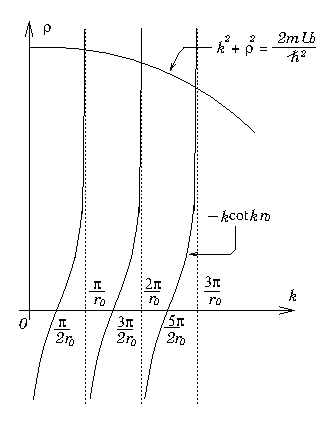
\includegraphics[clip,height=55mm,width=50mm]{1997phy1-1-2.eps}
\end{center}
}

\end{subsubanswers}

\SubAnswer
\begin{subsubanswers}

\SubSubAnswer
粒子の運動エネルギー$E$を無視した$r\leq r_0$における動径方程式($l=0$)を {\bf{1.(i),(ii)}}と同様に
$u_0(r)(=rR_0(r))$を用いて書くと、
\begin{equation}
\frac{d^2}{dr^2}u_0(r)+\frac{2m\alpha}{\hbar^2 r_0^2}u_0(r)=0\eqname{A9}
\end{equation}
$r=0$で$R_0(r)$が有界であるという条件のもとに解くと、
\begin{equation}
R_0(r)=\frac{u_0(r)}{r}=A\frac{\sin(\sqrt{\beta}\frac{r}{r_0})}{r}\eqname{A10}
\end{equation}
となる。但し、$\beta=2m\alpha/\hbar^2$である。

\SubSubAnswer
$R_0(r)\simeq r^{a}$を与えられた動径波動方程式に代入すると、$r^{a-2}$の係数について以下の関係が成り立つ。
\begin{equation}
a(a-1)+2a+\beta=0 \Longleftrightarrow a=-\frac{1}{2}\pm\sqrt{\frac{1}{4}-\beta}
\eqname{A11}
\end{equation}
従って、$\delta=\sqrt{\frac{1}{4}-\beta}$とおくと、$r\simeq r_0(r\geq r_0)$での近似的な動径関数は、
\begin{equation}
R_0(r)=Br^{-\frac{1}{2}+\delta}+Cr^{-\frac{1}{2}-\delta} 
\eqname{A12}
\end{equation}

\SubSubAnswer
\hspace{2mm}{\bf{2.(ii)}}で得られた動径波動関数の定数$B$、$C$の関係を$r=r_0$での接続条件から求める。\eqhref{A10}式と\eqhref{A12}式の\\
$u_0(r)=rR_0(r)$についての$r=r_0$における対数微分が等しいことより、
\begin{eqnarray}
\frac{\sqrt{\beta}}{r_0}\cot\sqrt{\beta} &=& \frac{(\frac{1}{2}-\delta)r_{0}^{-\frac{1}{2}-\delta}(Br_0^{2\delta}+C)
+r_0^{\frac{1}{2}-\delta}(2B\delta r_0^{2\delta-1})}{r_0^{\frac{1}{2}-\delta}(Br_0^{2\delta}+C)} \eqname{A13} \\
              &=& \frac{1}{r_0}\left(\frac{1}{2}-\delta\right)+\frac{2\delta r_0^{2\delta-1}}{r_0^{2\delta}+D}\eqname{A14}
\end{eqnarray}
但し、$D=C/B$とした。$D$について解くと、
\begin{equation}
D=-r_0^{2\delta}\frac{\sqrt{\beta}\cot\sqrt{\beta}-(\delta+\frac{1}{2})}{\sqrt{\beta}\cot\sqrt{\beta}+(\delta-\frac{1}{2})}\eqname{A15}
\end{equation}
となる。これより、定数を一つ減らすことができた。
\begin{equation}
R_0(r)=B\Biggl[r^{-\frac{1}{2}+\delta}-r_0^{2\delta}\frac{\sqrt{\beta}\cot\sqrt{\beta}-(\delta+\frac{1}{2})}{\sqrt{\beta}\cot\sqrt{\beta}+(\delta-\frac{1}{2})} r^{-\frac{1}{2}-\delta}\Biggr]\eqname{A16}
\end{equation}

\SubSubAnswer
$\beta\ge 1/4$の時、$\delta$は虚数となる。$\delta=i\varepsilon(\varepsilon\ge 0)$とすると、$r\geq r_0$において
\begin{equation}
R_0(r)=B\Biggl[r^{-\frac{1}{2}+i\varepsilon}-r_0^{2i\varepsilon}\frac{\sqrt{\beta}\cot\sqrt{\beta}-\frac{1}{2}-i\varepsilon}{\sqrt{\beta}\cot\sqrt{\beta
}-\frac{1}{2}+i\varepsilon}r^{-\frac{1}{2}-i\varepsilon}\Biggr] \eqname{A17}
\end{equation}
となり、$R_0(r)=0$は以下の形に書ける。
\begin{equation}
\Bigl(\frac{r}{r_0}\Bigr)^{2i\varepsilon}=\frac{\sqrt{\beta}\cot\sqrt{\beta}-\frac{1}{2}-i\varepsilon}{\sqrt{\beta}\cot\sqrt{\beta}-\frac{1}{2}+i\varepsilon}\eqname{A18}
\end{equation}
$\alpha^{x}=e^{x\ln \alpha}$などを用いて、実部と虚部に分けて両辺を比較すると、$K=\sqrt{\beta}\cot\sqrt{\beta}$を用いて
\begin{eqnarray}
\cos\left(2\varepsilon\ln{\frac{r}{r_0}}\right)&=&\frac{(K-\frac{1}{2})^2-\varepsilon^2}{(K-\frac{1}{2})^2+\varepsilon^2}\\
\sin\left(2\varepsilon\ln{\frac{r}{r_0}}\right)&=&-\frac{2\varepsilon(K-\frac{1}{2})^2}{(K-\frac{1}{2})^2+\varepsilon^2}\eqname{A19}
\end{eqnarray}
となる。$\beta$を一意に定めると上式の右辺は定数となり、$r$の満たすべき関係式は
\begin{equation}
2\varepsilon\ln{\frac{r}{r_0}}=\alpha_0+2n\pi\hspace{0.5cm}(n:整数,\alpha_0:定数)\eqname{A20}
\end{equation}
この関係は$r\simeq r_0$に限って近似的に成り立つものであり、$r_0>0$の時には上式を満たす$r$の数は有限個であると
考えられる。しかしながら、
$r_0\rightarrow\infty$の極限では、${\displaystyle{\lim_{r_0\rightarrow 0}\ln r_0=-\infty}}$の発散により、\eqhref{A20}式を満たす$r(\simeq r_0)$は定まらない。ここにおいて、束縛状態は無限に深い井戸の底(基底状態というものが定義できない)から詰まって、
無限個存在することになる。この原因は、$1/r^2$に比例するポテンシャル(問題で$r_0\rightarrow 0$としたもの)が、Heisenbergの不確定性関係に抵触して基底状態を持つことができないということにある。(詳しくは補足参照)


\end{subsubanswers}

[補足]: Hamiltonian:
\begin{equation}
H=\frac{\vec{p}^{\hspace{1mm} 2}}{2m}+\alpha r^{s}
\end{equation}
に対して、基底状態がHeisenbergの不確定性関係$\Delta p\cdot\Delta r\geq\hbar/2$を満たすための$s$の条件を調べる。基底状態
では不確定性が最小限であるとして、$p\simeq \hbar/2a$($a$:ポテンシャルの到達距離で波動関数の広がりに相当)とする。この時、基底状態のエネルギーは、
\begin{equation}
E_0\simeq \frac{1}{2m}\left(\frac{\hbar}{2a}\right)^2+\alpha a^{s}
\end{equation}
と書ける。$E_0$がエネルギー固有値であるためにはパラメーター$a$に対して安定でなければならない。このことから、
\begin{equation}
\frac{\partial E_0}{\partial a}=0 \Longleftrightarrow a=\left(\frac{\hbar^2}{16m\alpha s}\right)^{\frac{1}{s+2}} \eqname{hoso1}
\end{equation}

\begin{equation}
\frac{\partial^2 E_0}{\partial a^2}>0 \Longleftrightarrow  s+2>0 \eqname{hoso2}
\end{equation}
但し、\eqhref{hoso2}の計算には\eqhref{hoso1}の結果得られた$a$を用いた。これより、ポテンシャル$\alpha/r^2$(本問での$r_0\rightarrow 0$の極限に対応)
はギリギリのところで基底状態が存在できないことが分かった。

\end{subanswers}

\end{answer}
\end{document}